\documentclass[12pt,a4paper]{article}
\usepackage{algorithm, algpseudocode, amsmath, amssymb, amsthm, bm, csquotes, emf, empheq, geometry, graphicx, hyperref, listings, mhchem, multirow, siunitx, slashbox, subcaption, upgreek}
\usepackage[italicdiff]{physics}
\usepackage[section]{placeins}
\usepackage[justification=centering]{caption}
\usepackage[column=O]{cellspace}
\usepackage[extrafootnotefeatures]{xepersian}
\hypersetup{colorlinks=true, urlcolor=cyan}

\title{تمرین سری یازده دینامیک غیرخطی و آشوب}
\author{صالح شاملو احمدی}
\date{۲۷ اردیبهشت ۱۴۰۲}

\settextfont{Yas}
\linespread{1.2}

\setlength\cellspacetoplimit{4pt}
\setlength\cellspacebottomlimit{3pt}
\newcommand{\multlinecell}[1]{\begin{tabular}[c]{@{}c@{}}#1\end{tabular}}

\newcommand{\qfrac}[2]{\left(\frac{#1}{#2}\right)}
\newcommand{\fsqrt}[2]{\sqrt{\frac{#1}{#2}}}
\newcommand{\ddfrac}[2]{{\displaystyle\frac{\displaystyle #1}{\displaystyle #2}}}
\newcommand{\pdvc}[3]{\qfrac{\partial #1}{\partial #2}_{#3}}
\newcommand{\dbar}{{d\mkern-7mu\mathchar'26\mkern-2mu}}
\newcommand*{\defeq}{\mathrel{\vcenter{\baselineskip0.5ex \lineskiplimit0pt
			\hbox{\scriptsize.}\hbox{\scriptsize.}}}
	=}

\newtheorem{theorem}{قضیه}
\newtheorem{lemma}{لم}
\renewcommand\qedsymbol{$\blacksquare$}

\begin{document}
	\maketitle
	\section{مسئله \lr{8.4.4}}
	\begin{subequations}
		\begin{empheq}[left=\empheqlbrace]{align}
			\dot{\theta} &= \dot{y} \\
			\dot{y} &= (\mu\cos\theta - 1)y - \sin\theta
		\end{empheq}
	\end{subequations}
	با خطی‌سازی،
	\begin{equation}
		J_{(x, y)} = \mqty(0 & 1 \\ -\mu y\sin\theta - \cos\theta & \mu\cos\theta - 1),
	\end{equation}
	پس در مبدأ
	\begin{equation}
		J_{(0, 0)} = \mqty(0 & 1 \\ -1 & \mu - 1).
	\end{equation}
	با استفاده از رد و دترمینان، ویژه مقادیر را بدست می‌آوریم.
	\begin{empheq}[left=\empheqlbrace, right={\implies \lambda^2 + (1-\mu)\lambda + 1 = 0}]{align}
		\tau &= \mu - 1 \\
		\Delta &= 1
	\end{empheq}
	\begin{equation}
		\lambda = \frac{\mu-1\pm\sqrt{\mu^2 - 2\mu - 3}}{2}
	\end{equation}
	\newgeometry{top=1in, bottom=1.5in}
	در $\mu=1 $ نقطه ثابت مبدأ از حالت پایدار به حالت ناپایدار تبدیل می‌شود. با توجه به رابطه مربوط به ویژه‌مقادیر آن،
	این یک دوشاخگی \lr{Hopf} می‌دهد، چراکه دو ویژه مقدار مختلط و با بخش حقیقی یکسان هستند که در $\mu = 1 $ از محور موهومی
	عبور می‌کنند. با حل عددی و رسم شکل فضای فاز، این دوشاخگی واضح می‌شود.

	\begin{figure}[h!]
		\centering
		\begin{subfigure}{0.49\linewidth}
			\centering
			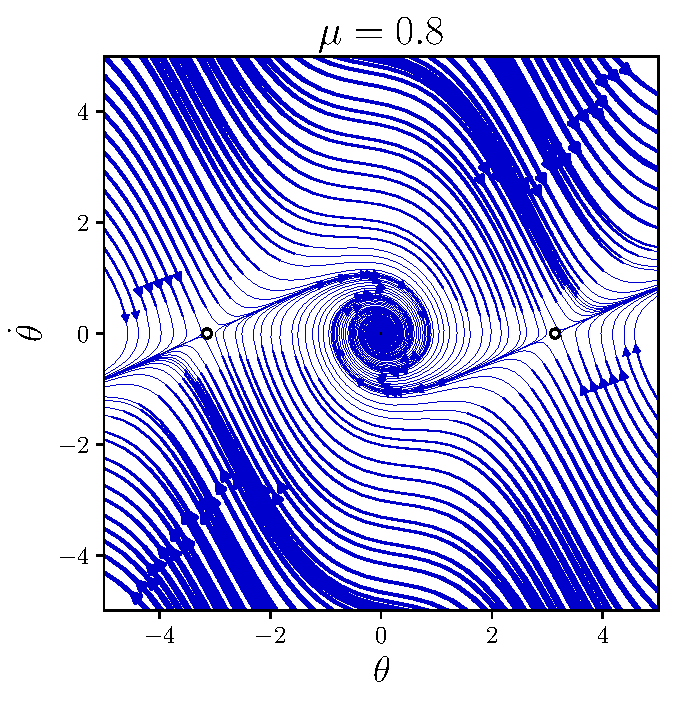
\includegraphics[width=\linewidth]{fig/8.4.4.mu0.8}
			\caption{قبل دوشاخگی}
		\end{subfigure}
		\begin{subfigure}{0.49\linewidth}
			\centering
			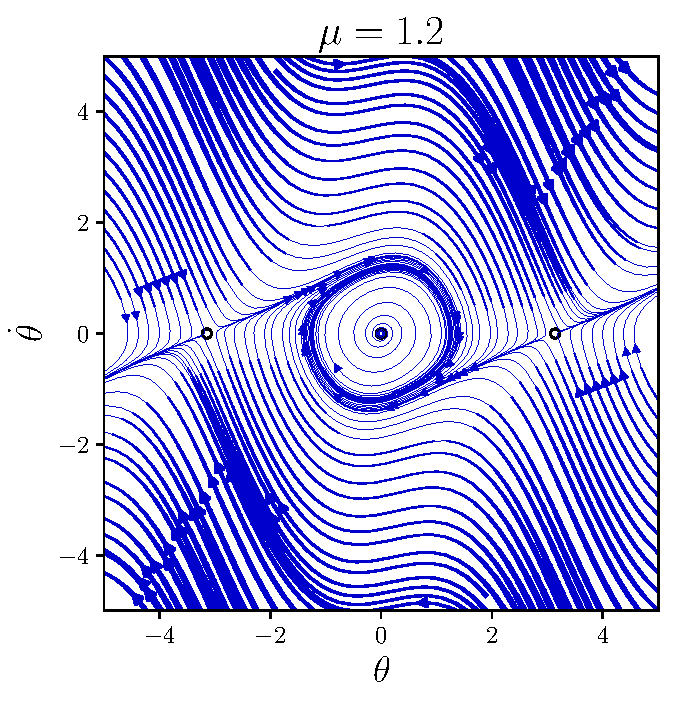
\includegraphics[width=\linewidth]{fig/8.4.4.mu1.2}
			\caption{بعد دوشاخگی}
		\end{subfigure}
		\begin{subfigure}{0.49\linewidth}
			\centering
			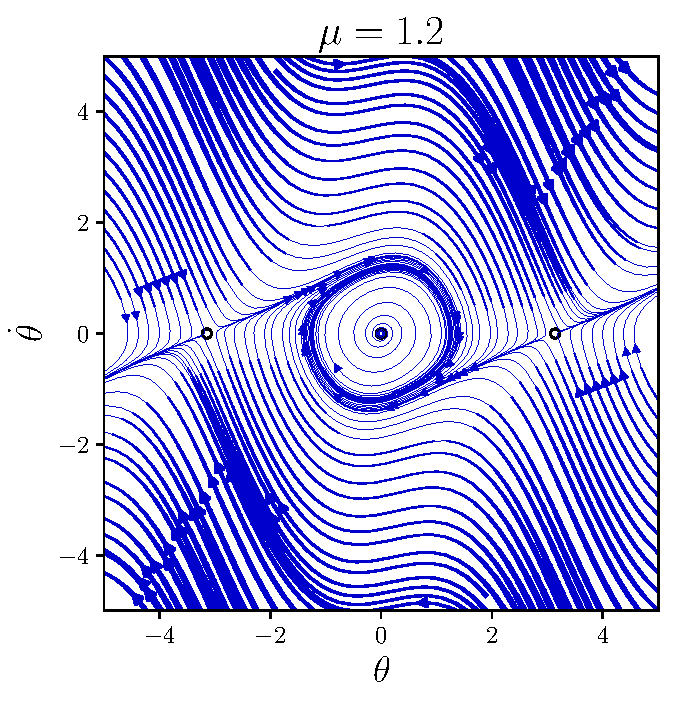
\includegraphics[width=\linewidth]{fig/8.4.4.mu1.2}
			\caption{روی دوشاخگی}
		\end{subfigure}
		\caption{دوشاخگی \lr{Hopf} در $\mu=1$}
	\end{figure}

	با افزایش $\mu$، چرخه حدی درست شده رشد می‌کند تا به نقاط ثابت $(\theta, \dot{\theta}) = (-\pi, 0)$
	و $(\theta, \dot{\theta}) = (\pi, 0)$ برسد و از بین برود. در جایی که این اتفاق می‌افتد، دوشاخگی هوموکلینیک داریم.
	با حل عددی به نظر می‌رسد مقدار $\mu$ در این دوشاخگی بین $3.72$ و $3.73$ است.
	
	\begin{figure}[h!]
		\centering
		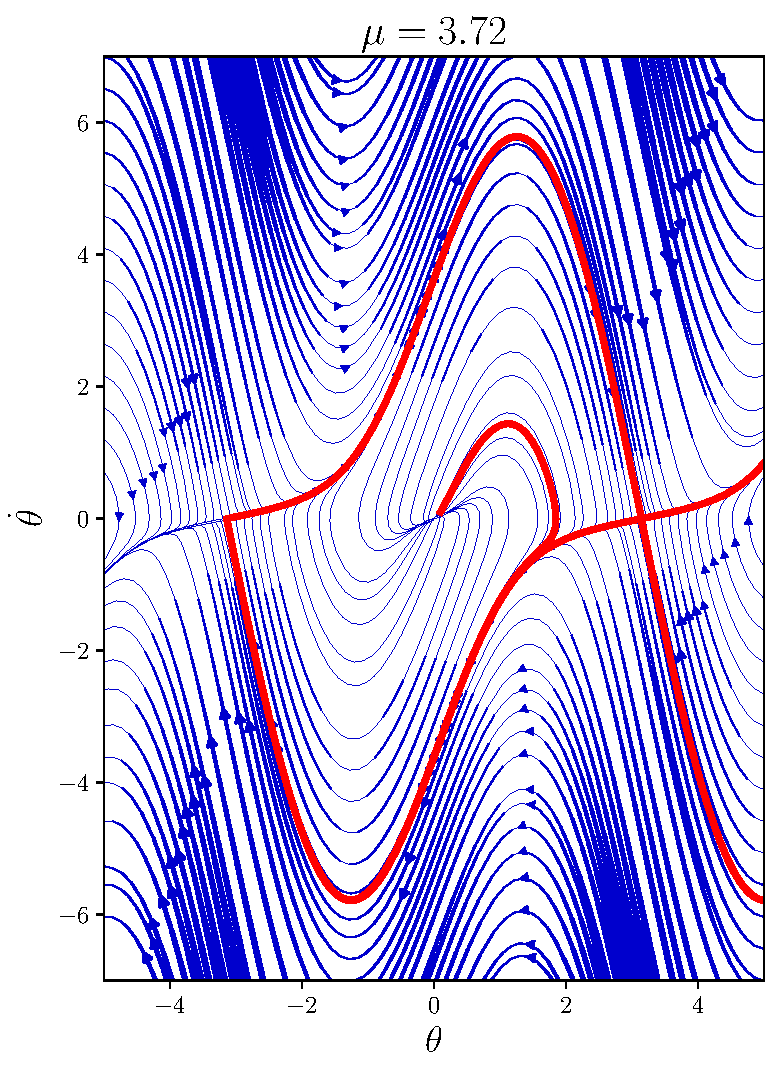
\includegraphics[width=\linewidth]{fig/8.4.4.mu3.72}
		\caption{قبل دوشاخگی هوموکلینیک}
	\end{figure}
	\begin{figure}[h!]
		\centering
		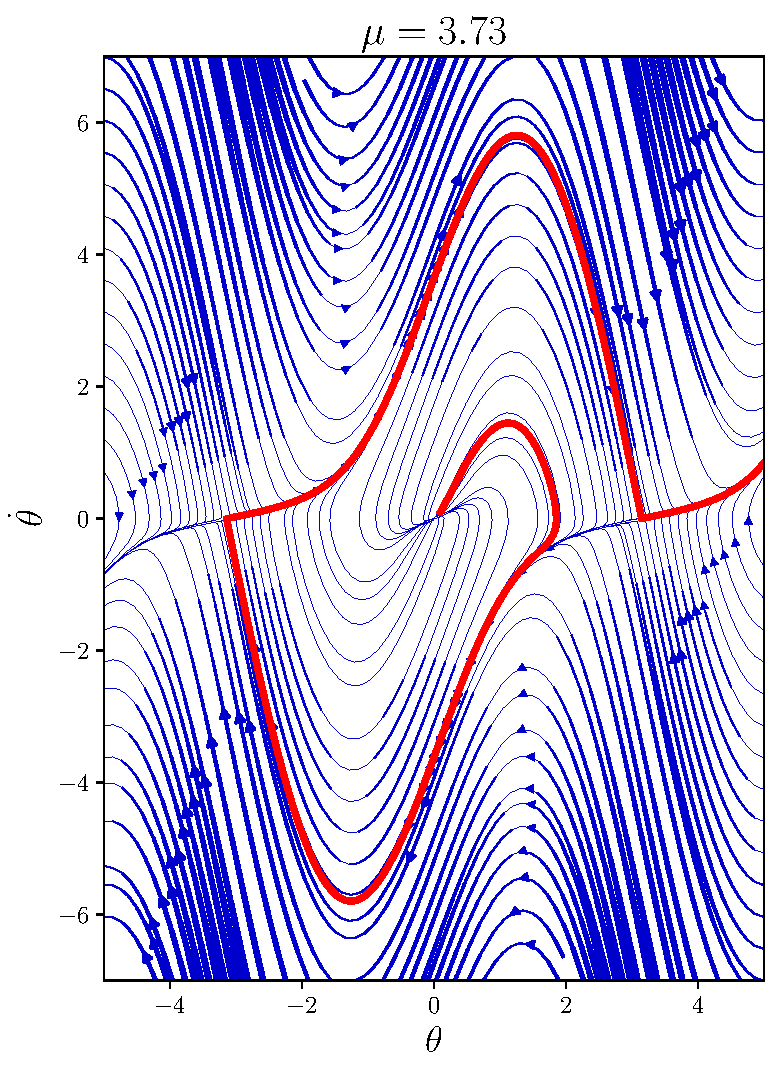
\includegraphics[width=\linewidth]{fig/8.4.4.mu3.73}
		\caption{بعد دوشاخگی هوموکلینیک}
	\end{figure}
	\restoregeometry
	\section{مسئله \lr{8.7.3}}
	\subsection{\lr{a}}
	\begin{align}
		x + \dot{x} = F(t) &\xRightarrow{\times e^{t}} xe^t + \dot{x}e^t = F(t)e^t \\
		\dv{xe^t}{t} = F(t) &\implies \int_0^T \dv{xe^t}{t} \dd{t} = \int_0^T F(t)e^t \dd{t} \\
		\eval{\qty(xe^t)}_0^T &= \int_{0}^{T/2}Ae^t\dd{t} - \int_{T/2}^T Ae^t\dd{t} \\
		x(T)e^T - x(0) &= A\qty(e^{T/2} - 1) - A\qty(e^T - e^{T/2}) \\
		x(T)e^T &= x_0 + A\qty(2e^{T/2} - e^T - 1) \\
		x(T) &= x_0e^{-T} - Ae^{-T}\qty(e^{T/2} - 1)^2 \\
		x(T) &= x_0e^{-T} - A\qty(1 - e^{-T/2})^2
	\end{align}
	\subsection{\lr{b}}
	شرط تناوبی بودن جواب، $x(T) = x(0)$ است. بنابراین با استفاده از نتیجه بخش قبل،
	\begin{equation}
		x(0)e^{-T} - A\qty(1 - e^{-T/2})^2 = x(0)
	\end{equation}
	\begin{align}
		x(0) &= -A\frac{\qty(1 - e^{-T/2})^2}{1-e^{-T}} \\
		&= -A\frac{e^{T/2}\qty(1 - e^{-T/2})^2}{e^{T/2}-e^{-T/2}} \\
		&= -A\frac{\qty(e^{T/4} - e^{-T/4})^2}{\qty(e^{T/4}-e^{-T/4})\qty(e^{T/4}+e^{-T/4})} \\
		&= -A\frac{e^{T/4} - e^{-T/4}}{e^{T/4}+e^{-T/4}} \\
		&= -A\tanh(\frac{T}{4}).
	\end{align}
	\subsection{\lr{c}}
	طبق نتیجه بخش \lr{a}،
	\begin{align}
		\lim_{T\to0}x(T) &= x_0, \\
		\lim_{T\to\infty}x(T) &= -A.
	\end{align}
	در حد $T\to0 $ عامل $F(t)$ زمان کافی برای تغییر $x$ را ندارد، بنابراین $x(t)\approx x_0 $.
	در حد $T\to\infty$ عامل $F(t)$ مقدار $x$ را به $-A$ می‌رساند و به دلیل بی‌نهایت بودن دوره تناوب، $x$ را همان‌جا
	نگه می‌دارد.
	\subsection{\lr{d \& e}}
	شرط لازم و کافی برای پایدار بودن نقطه ثابت نگاشت پوانکاره، کمتر بودن شیب خط $P(x)$ از $1$ در نقطه ثابت
	(تقاطع $y = P(x)$ و $y = x$) است. از طرفی
	\begin{equation}
		P(x) = xe^{-T} - A\qty(1-e^{-T/2})
	\end{equation}
	که به ازای مقادیر مثبت برای $T$ و $A$ همواره خطی با شیب کمتر از یک و عرض از مبدأ منفی است. بنابراین نقطه
	\begin{equation}
		P(x^*) = x^* \implies x^* = -A\tanh(\frac{T}{4})
	\end{equation}
	(از نتیجه بخش ب) یک نقطه ثابت پایدار برای نگاشت پوانکاره است. همچنین به دلیل یکنوا بودن نگاشت پوانکاره برحسب $x$،
	این تنها نقطه ثابت و به‌صورت سراسری پایدار است.
	\begin{figure}[h!]
		\centering
		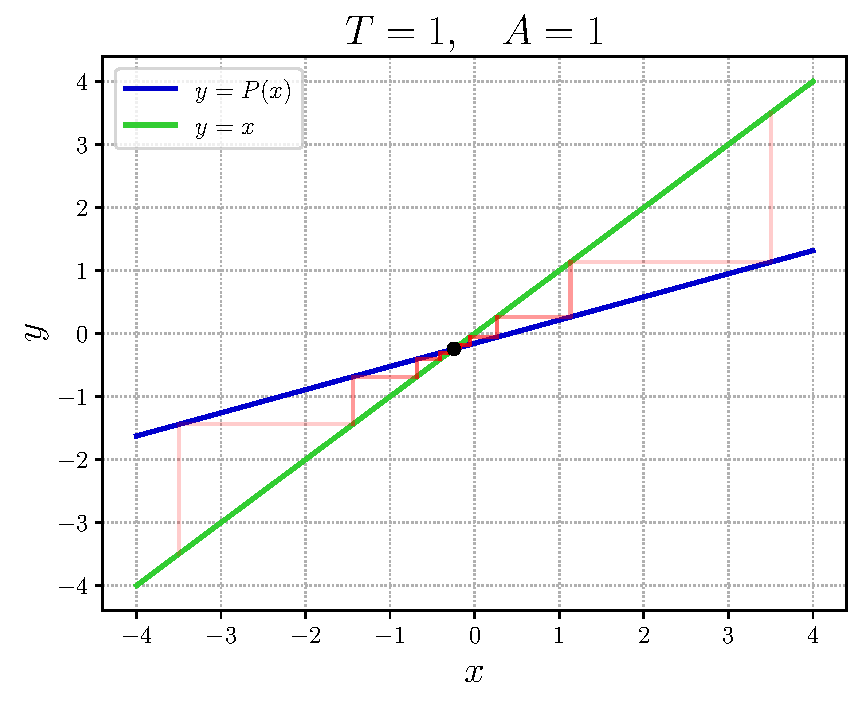
\includegraphics[width=\linewidth]{fig/8.7.3}
		\caption{نمودار تارعنکبوتی. خط‌ها با بالا رفتن تعداد قدم $n$ به تدریج پررنگ می‌شوند.}
	\end{figure}
	\section{مسئله \lr{9.3.9}}
	با فیت کردن خط‌های متعدد به فاصله مسیرها در شرایط اولیه متفاوت و میانگین‌گیری از شیب‌ها، مقدار $\lambda$
	را بدست می‌آوریم؛ شرایظ اولیه
	$\qty(x_0, y_0, z_0) = (0.896, 1.561, 11.264)$
	را انتخاب می‌کنیم (از آن استفاده می‌کنیم چون در ابتدای مسیر اختلال کمتری دارد). سپس مسیر دیگری با شرایط اولیه‌ای
	در کره‌ای با شعاع $0.001$ حول نقطه اول به صورت تصادفی انتخاب می‌کنیم. این مراحل را به دفعات زیادی تکرار می‌کنیم
	تا $\lambda$ «اصلی» را بدست بیاوریم. با این روش $\lambda$ حدود $0.956$ بدست می‌آید که همچنان اختلاف به نسبت زیادی با
	مقدار اصلی که $0.906$ است دارد که به دلیل اختلال بالای مسئله است.
	\begin{figure}[h!]
		\centering
		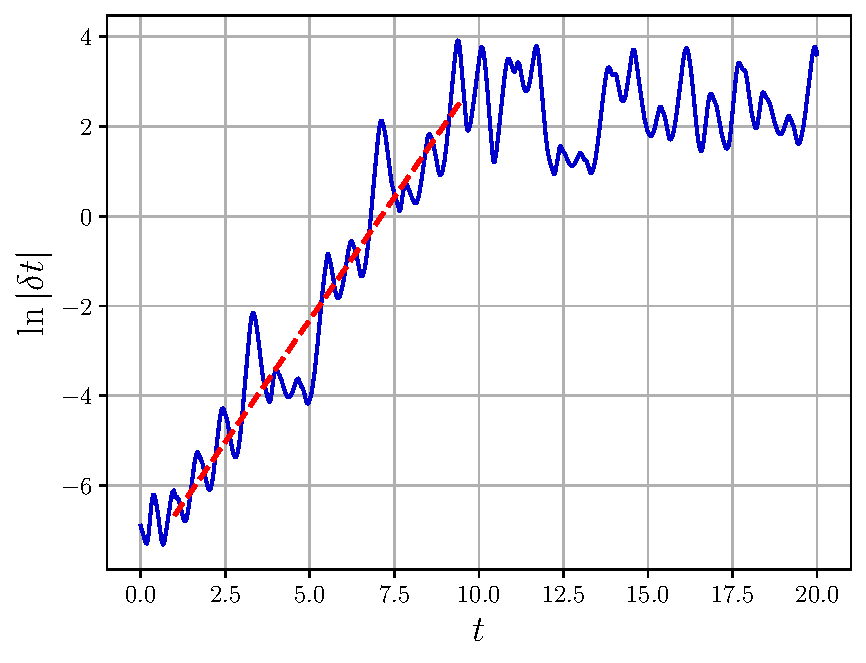
\includegraphics[width=\linewidth]{fig/9.3.9}
		\caption{نمونه فیت که روی بازه به نسبت خطی انجام شده.}
	\end{figure}
\end{document}